\section{Empirical Validation}
\label{sec:experiments}

We evaluate the impact of using \sysname to train Transformer models.
\begin{itemize}[itemsep=0.1pt,topsep=0pt,leftmargin=*]
  \item \textbf{Benchmarking attention.}
  We measure the runtime of \sysname across different sequence lengths and
  compare it to a standard implementation in PyTorch, \sysnameone, and
  \sysnameone in Triton.
  We confirm that \sysname is 1.7-3.0$\times$ faster than \sysnameone, 1.3-2.5$\times$
  faster than \sysnameone in Triton, and 3-10$\times$ faster than a standard
  attention implementation.
  \sysname reaches up to 230 TFLOPs/s, 73\% of the theoretical maximum TFLOPs/s
  on A100 GPUs.
  \item \textbf{End-to-end training speed}
  When used end-to-end to train GPT-style models of size 1.3B and 2.7B on
  sequence lengths either 2k or 8k, \sysname yields up to 1.3$\times$ speedup compared to
  \sysnameone and 2.8$\times$ speedup compared to a baseline without \sysnameone.
  \sysname reaches up to 225 TFLOPs/s (72\% model FLOPs utilization) per A100 GPU.
\end{itemize}

\subsection{Benchmarking Attention}
\label{subsec:benchmark_attn}

We measure the runtime of different attention methods on an A100 80GB SXM4 GPU
for different settings (without / with causal mask, head dimension 64 or 128).
We report the results
in~\cref{fig:benchmark_attn_fwd_bwd},~\cref{fig:benchmark_attn_fwd}
and~\cref{fig:benchmark_attn_bwd}, showing that \sysname is around 2$\times$ faster
than \sysnameone and \sysnameone in \texttt{xformers} (the ``cutlass''
implementation).
\sysname is around 1.3-1.5$\times$ faster than \sysnameone in Triton in the forward
pass and around 2$\times$ faster in the backward pass.
Compared to a standard attention implementation in PyTorch, \sysname can be up
to 10$\times$ faster.

Benchmark setting: we vary the sequence length from 512, 1k, ..., 16k, and set
batch size so that the total number of tokens is 16k.
We set hidden dimension to 2048, and head dimension to be either 64 or 128
(i.e., 32 heads or 16 heads).
To calculate the FLOPs of the forward pass, we use:
\begin{equation*}
  4 \cdot \text{seqlen}^2 \cdot \text{head dimension} \cdot \text{number of heads}.
\end{equation*}
With causal mask, we divide this number by 2 to account for the fact that
approximately only half of the entries are calculated.
To get the FLOPs of the backward pass, we multiply the forward pass FLOPs by 2.5
(since there are 2 matmuls in the forward pass and 5 matmuls in the backward
pass, due to recomputation).

\begin{figure}[ht]
  \centering
  \begin{subfigure}{.5\textwidth}
    \centering
    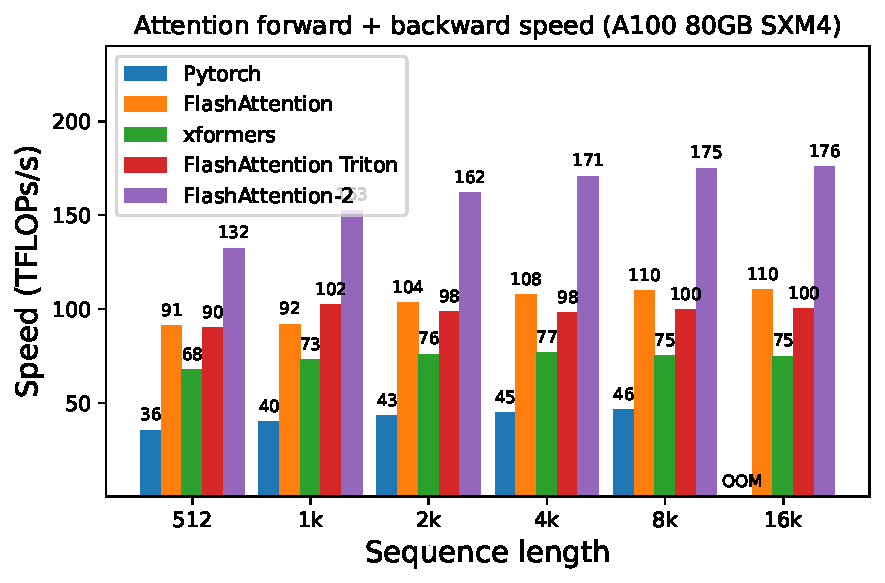
\includegraphics[width=.95\linewidth]{figs/flash2_causal_False_hdim_64_fwd_bwd_speed.pdf}
    \caption{Without causal mask, head dimension 64}
  \end{subfigure}%
  \begin{subfigure}{.5\textwidth}
    \centering
    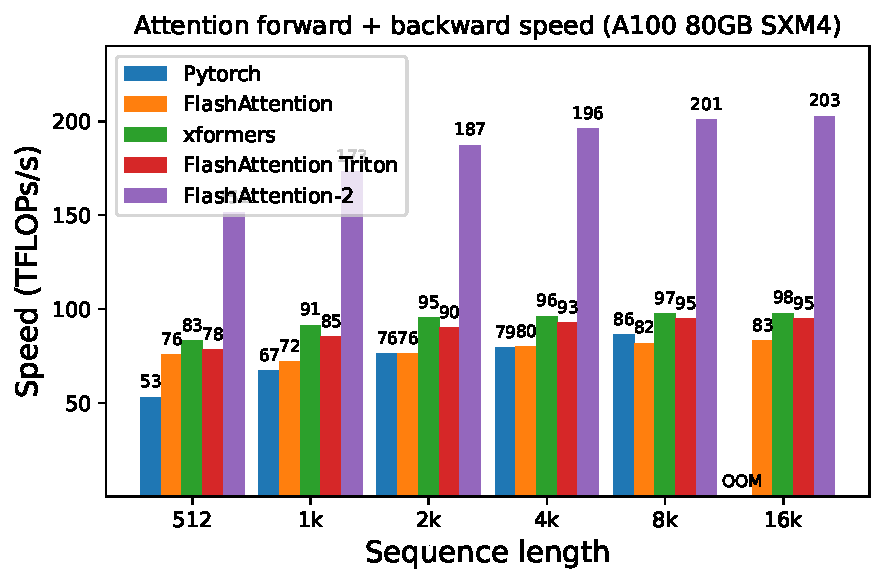
\includegraphics[width=.95\linewidth]{figs/flash2_causal_False_hdim_128_fwd_bwd_speed.pdf}
    \caption{Without causal mask, head dimension 128}
  \end{subfigure}
  \begin{subfigure}{.5\textwidth}
    \centering
    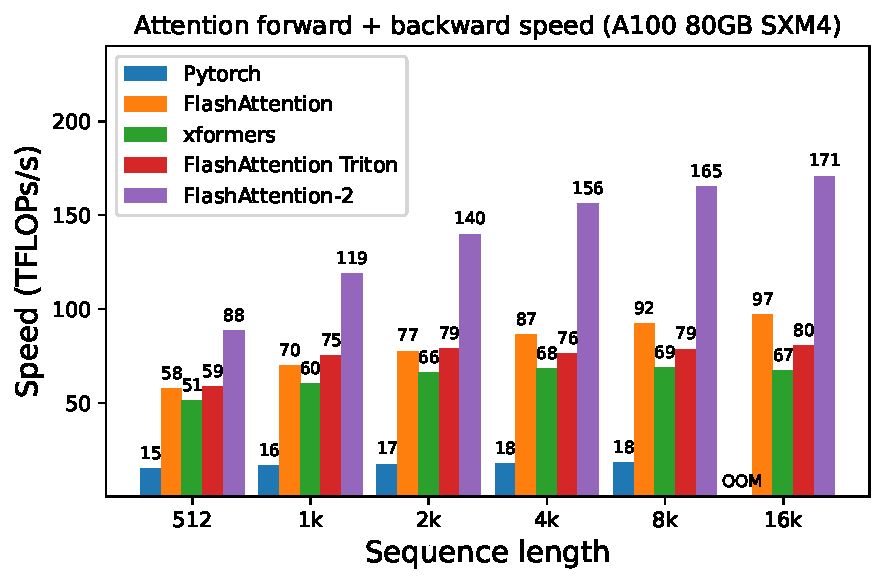
\includegraphics[width=.95\linewidth]{figs/flash2_causal_True_hdim_64_fwd_bwd_speed.pdf}
    \caption{With causal mask, head dimension 64}
  \end{subfigure}%
  \begin{subfigure}{.5\textwidth}
    \centering
    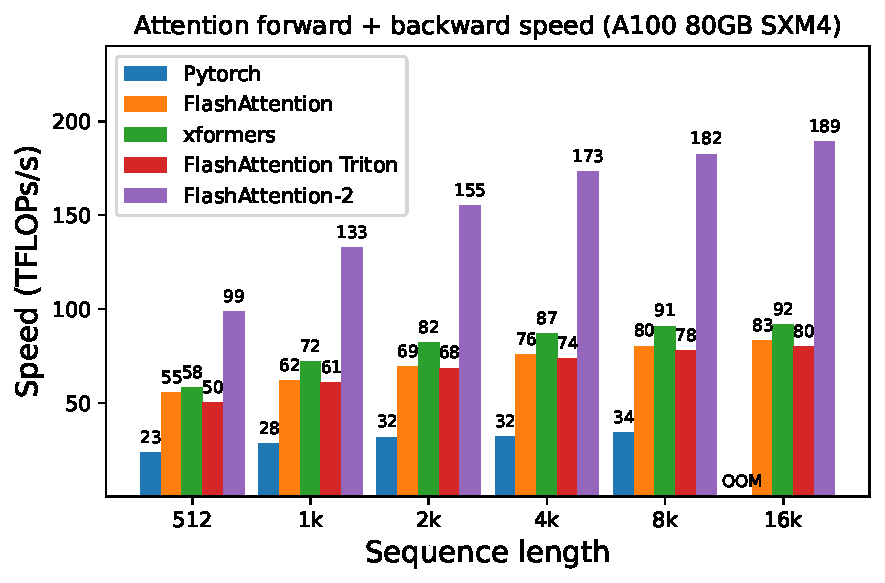
\includegraphics[width=.95\linewidth]{figs/flash2_causal_True_hdim_128_fwd_bwd_speed.pdf}
    \caption{With causal mask, head dimension 128}
  \end{subfigure}
  \caption{Attention forward + backward speed on A100 GPU}
  \label{fig:benchmark_attn_fwd_bwd}
\end{figure}

\begin{figure}[ht]
  \centering
  \begin{subfigure}{.5\textwidth}
    \centering
    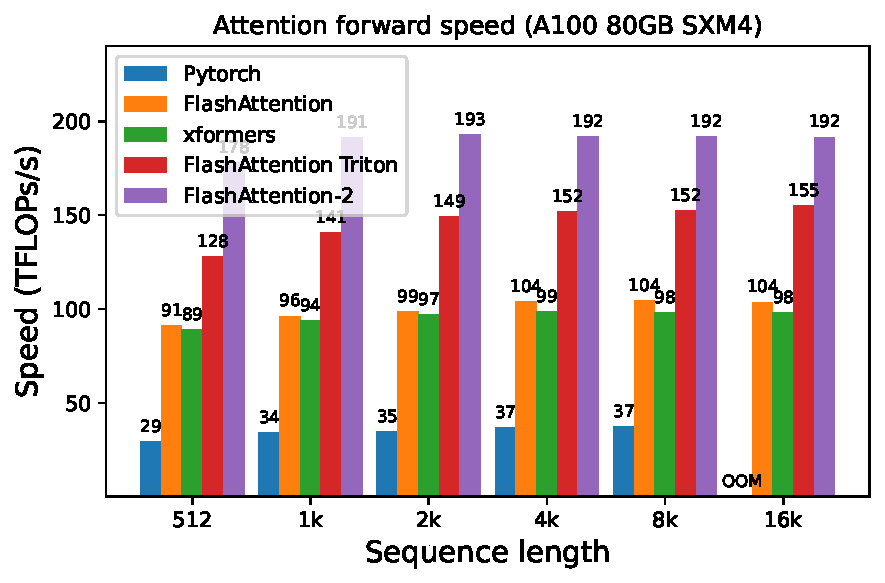
\includegraphics[width=.95\linewidth]{figs/flash2_causal_False_hdim_64_fwd_speed.pdf}
    \caption{Without causal mask, head dimension 64}
  \end{subfigure}%
  \begin{subfigure}{.5\textwidth}
    \centering
    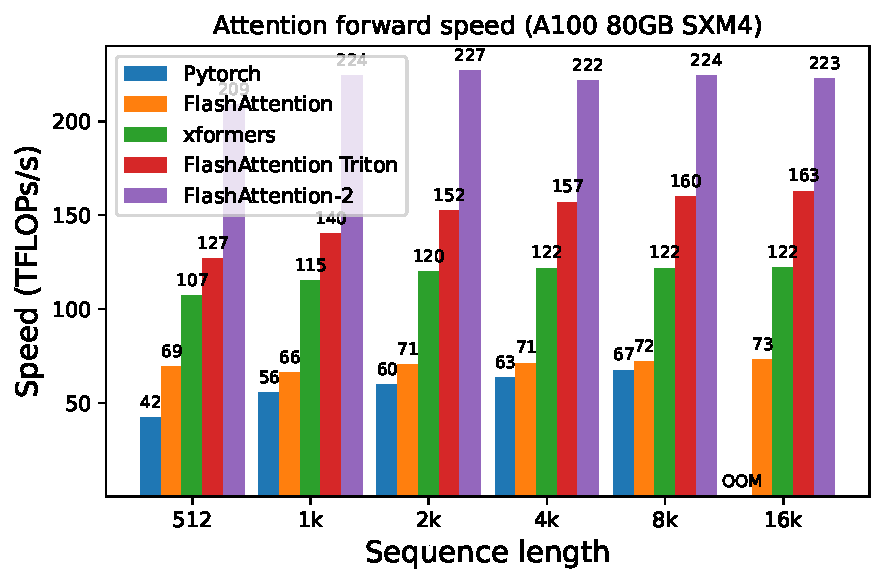
\includegraphics[width=.95\linewidth]{figs/flash2_causal_False_hdim_128_fwd_speed.pdf}
    \caption{Without causal mask, head dimension 128}
  \end{subfigure}
  \begin{subfigure}{.5\textwidth}
    \centering
    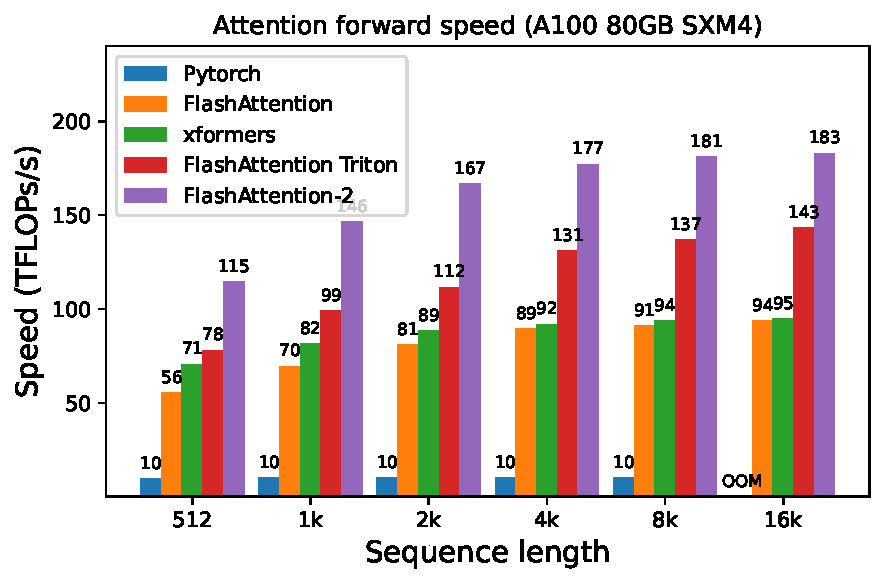
\includegraphics[width=.95\linewidth]{figs/flash2_causal_True_hdim_64_fwd_speed.pdf}
    \caption{With causal mask, head dimension 64}
  \end{subfigure}%
  \begin{subfigure}{.5\textwidth}
    \centering
    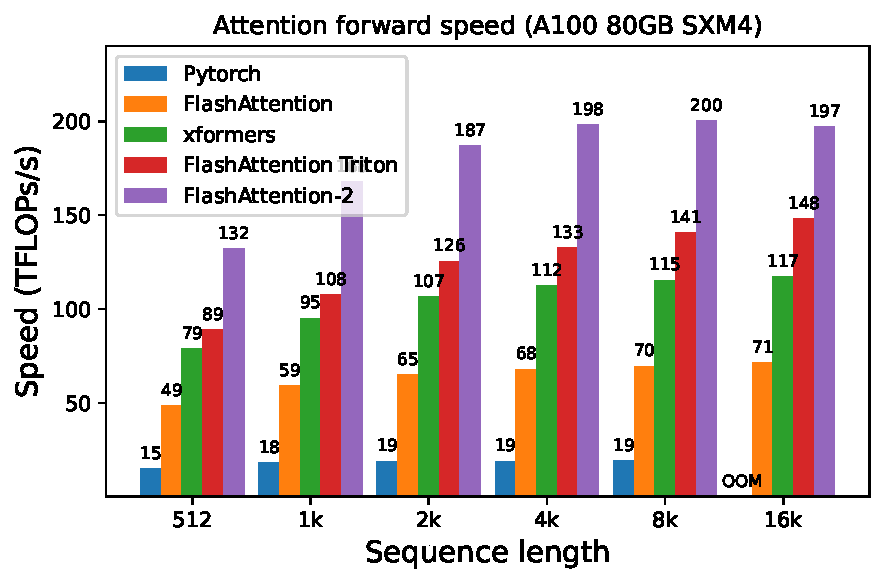
\includegraphics[width=.95\linewidth]{figs/flash2_causal_True_hdim_128_fwd_speed.pdf}
    \caption{With causal mask, head dimension 128}
  \end{subfigure}
  \caption{Attention forward speed on A100 GPU}
  \label{fig:benchmark_attn_fwd}
\end{figure}

\begin{figure}[ht]
  \centering
  \begin{subfigure}{.5\textwidth}
    \centering
    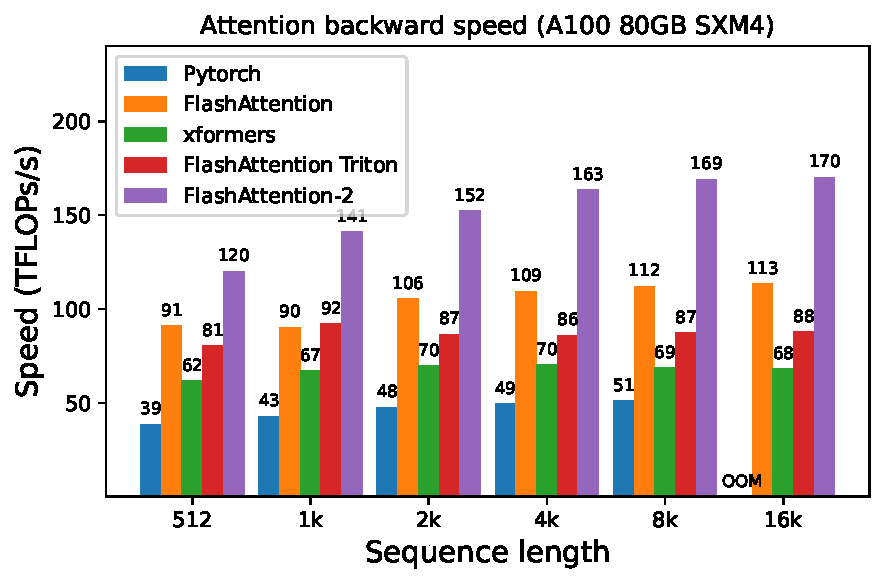
\includegraphics[width=.95\linewidth]{figs/flash2_causal_False_hdim_64_bwd_speed.pdf}
    \caption{Without causal mask, head dimension 64}
  \end{subfigure}%
  \begin{subfigure}{.5\textwidth}
    \centering
    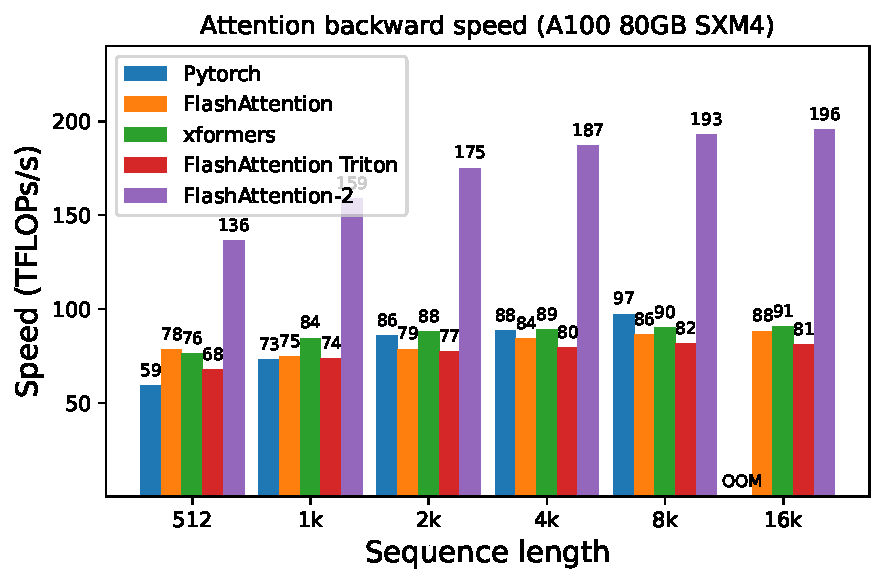
\includegraphics[width=.95\linewidth]{figs/flash2_causal_False_hdim_128_bwd_speed.pdf}
    \caption{Without causal mask, head dimension 128}
  \end{subfigure}
  \begin{subfigure}{.5\textwidth}
    \centering
    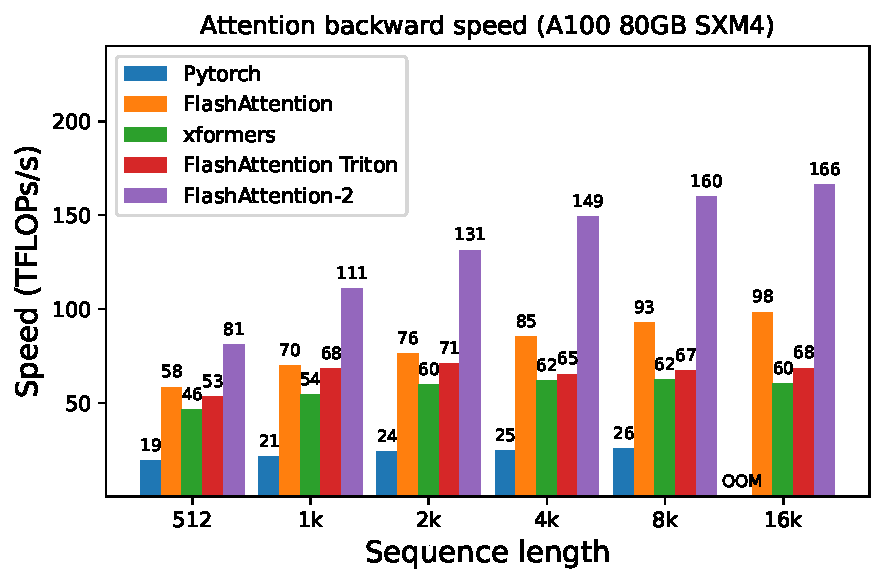
\includegraphics[width=.95\linewidth]{figs/flash2_causal_True_hdim_64_bwd_speed.pdf}
    \caption{With causal mask, head dimension 64}
  \end{subfigure}%
  \begin{subfigure}{.5\textwidth}
    \centering
    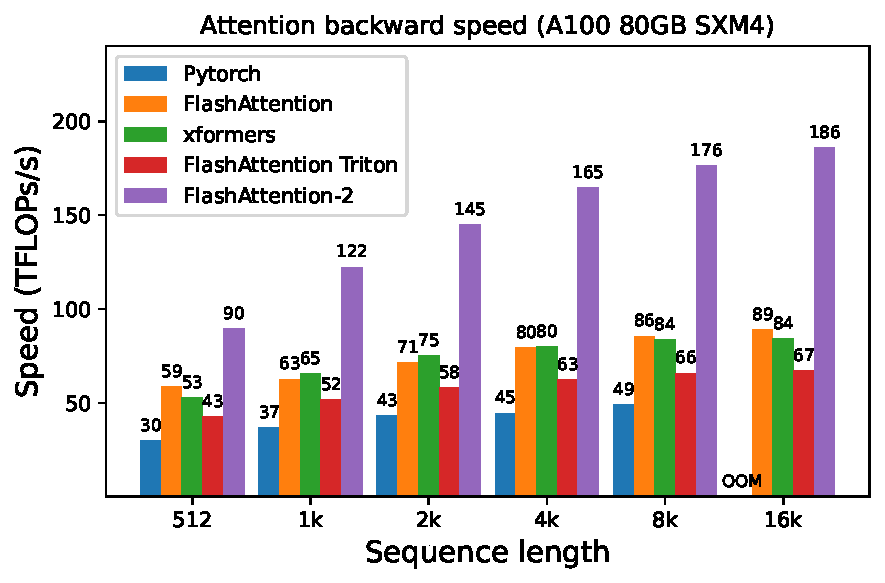
\includegraphics[width=.95\linewidth]{figs/flash2_causal_True_hdim_128_bwd_speed.pdf}
    \caption{With causal mask, head dimension 128}
  \end{subfigure}
  \caption{Attention backward speed on A100 GPU}
  \label{fig:benchmark_attn_bwd}
\end{figure}

Just running the same implementation on H100 GPUs (using no special instructions
to make use of new features such as TMA and 4th-gen Tensor Cores), we obtain up
to 335 TFLOPs/s (\cref{fig:benchmark_attn_fwd_bwd_h100}).
We expect that by using new instructions, we can obtain another 1.5x-2x speedup
on H100 GPUs. We leave that to future work.

\begin{figure}[ht]
  \centering
  \begin{subfigure}{.5\textwidth}
    \centering
    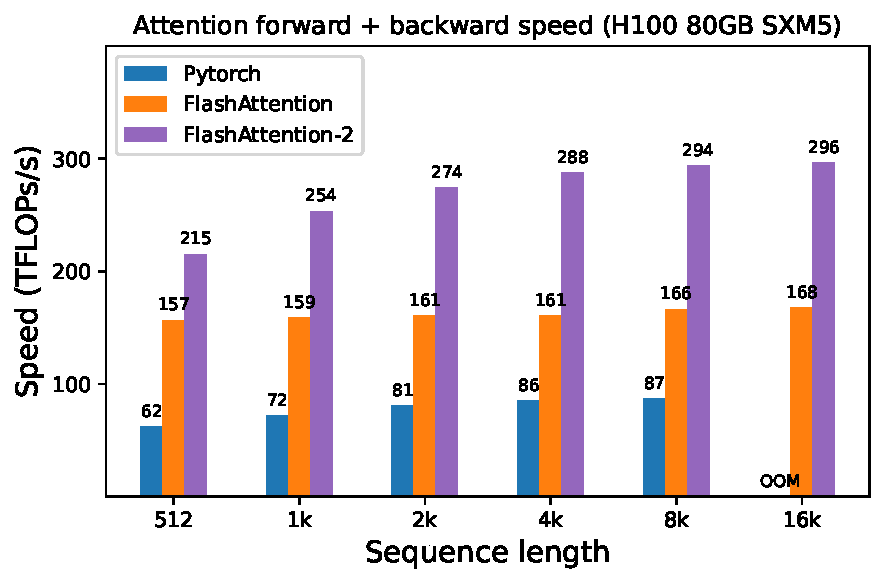
\includegraphics[width=.95\linewidth]{figs/flash2_h100_causal_False_hdim_64_fwd_bwd_speed.pdf}
    \caption{Without causal mask, head dimension 64}
  \end{subfigure}%
  \begin{subfigure}{.5\textwidth}
    \centering
    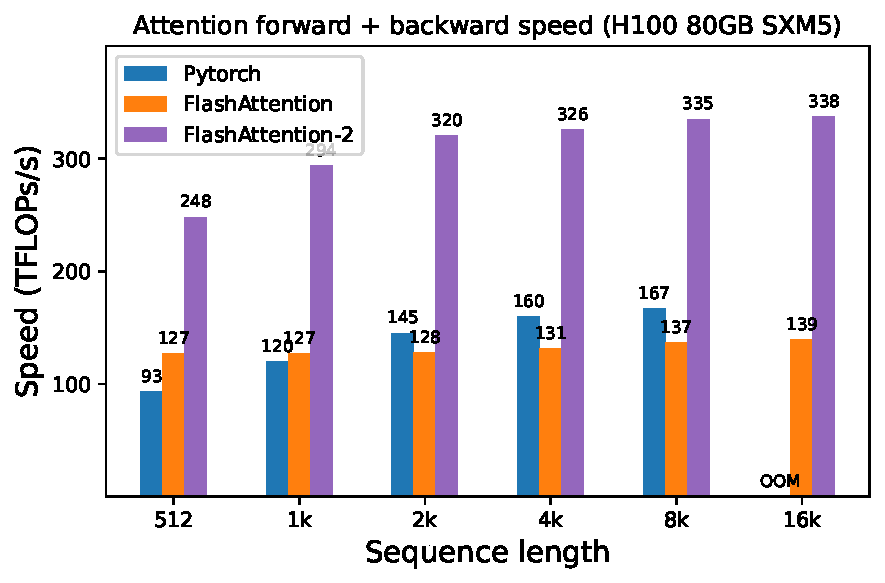
\includegraphics[width=.95\linewidth]{figs/flash2_h100_causal_False_hdim_128_fwd_bwd_speed.pdf}
    \caption{Without causal mask, head dimension 128}
  \end{subfigure}
  \begin{subfigure}{.5\textwidth}
    \centering
    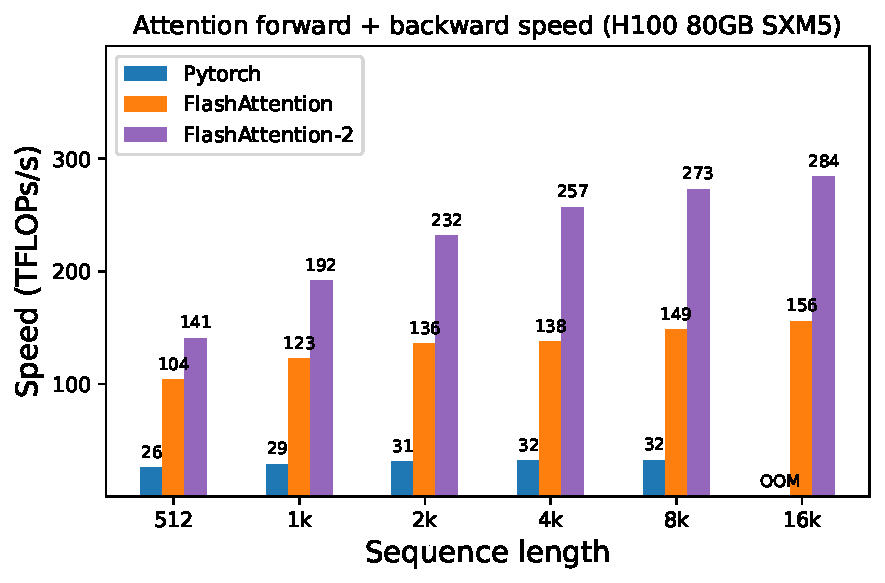
\includegraphics[width=.95\linewidth]{figs/flash2_h100_causal_True_hdim_64_fwd_bwd_speed.pdf}
    \caption{With causal mask, head dimension 64}
  \end{subfigure}%
  \begin{subfigure}{.5\textwidth}
    \centering
    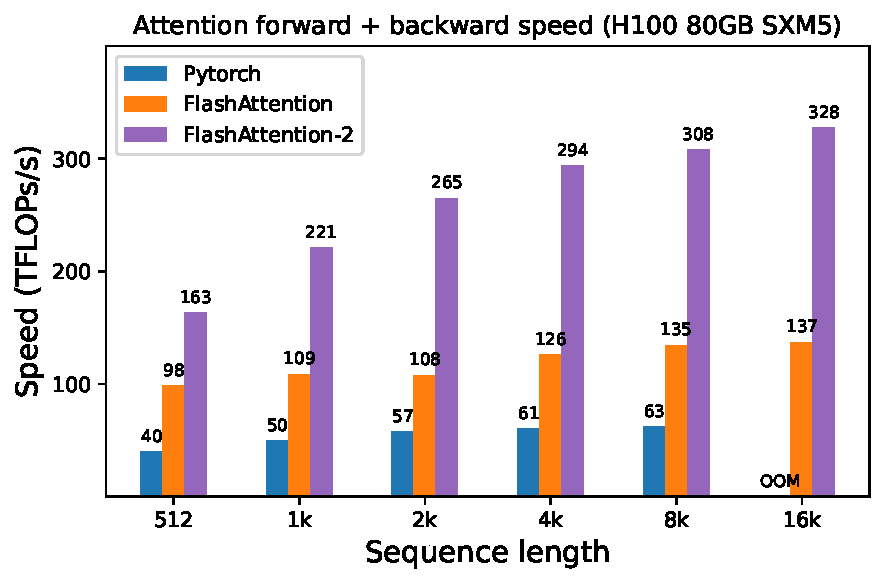
\includegraphics[width=.95\linewidth]{figs/flash2_h100_causal_True_hdim_128_fwd_bwd_speed.pdf}
    \caption{With causal mask, head dimension 128}
  \end{subfigure}
  \caption{Attention forward + backward speed on H100 GPU}
  \label{fig:benchmark_attn_fwd_bwd_h100}
\end{figure}

\subsection{End-to-end Performance}
\label{subsec:end_to_end}

We measure the training throughput of GPT-style models with either 1.3B or 2.7B
parameters, on 8$\times$A100 80GB SXM.
As shown in \cref{table:end_to_end}, \sysname yields 2.8$\times$ speedup compared to
a baseline without FlashAttention and 1.3$\times$ speedup compared to \sysname, reaching up to 225 TFLOPs/s
per A100 GPU.

Note that we calculate the FLOPs by the formula, following Megatron-LM~\citep{shoeybi2019megatron} (and many
other papers and libraries):
\begin{equation*}
  6 \cdot \text{seqlen} \cdot \text{number of params} + 12 \cdot \text{number of
    layers} \cdot \text{hidden dim} \cdot \text{seqlen}^2.
\end{equation*}
The first term accounts for the FLOPs due to weight--input multiplication, and
the second term accounts for the FLOPs due to attention.
However, one can argue that the second term should be halved, as with causal
mask we only need to compute approximately half the number of elements in
attention.
We choose to follow the formula from the literature (without dividing the
attention FLOPs by 2) for consistency.

\begin{table}[h!]
  \centering
  \caption{\label{table:end_to_end}Training speed (TFLOPs/s/GPU) of GPT-style
    models on 8$\times$A100 GPUs.
    \sysname reaches up to 225 TFLOPs/s (72\% model FLOPs utilization).
    We compare against a baseline running without \sysnameone.
  }
    {
      \begin{tabular}{@{}c|ccc@{}}
        Model & Without \sysnameone & \sysnameone & \sysname \\ \hline
        GPT3-1.3B 2k context & 142 TFLOPs/s & 189 TFLOPs/s & 196 TFLOPs/s \\
        GPT3-1.3B 8k context & 72 TFLOPS/s & 170 TFLOPs/s & 220 TFLOPs/s \\
        GPT3-2.7B 2k context & 149 TFLOPs/s & 189 TFLOPs/s & 205 TFLOPs/s \\
        GPT3-2.7B 8k context & 80 TFLOPs/s & 175 TFLOPs/s & 225 TFLOPs/s \\
      \end{tabular}
    }
  \end{table}




%%% Local Variables:
%%% mode: latex
%%% TeX-master: "../flash2"
%%% End:
